\chapter{后记}

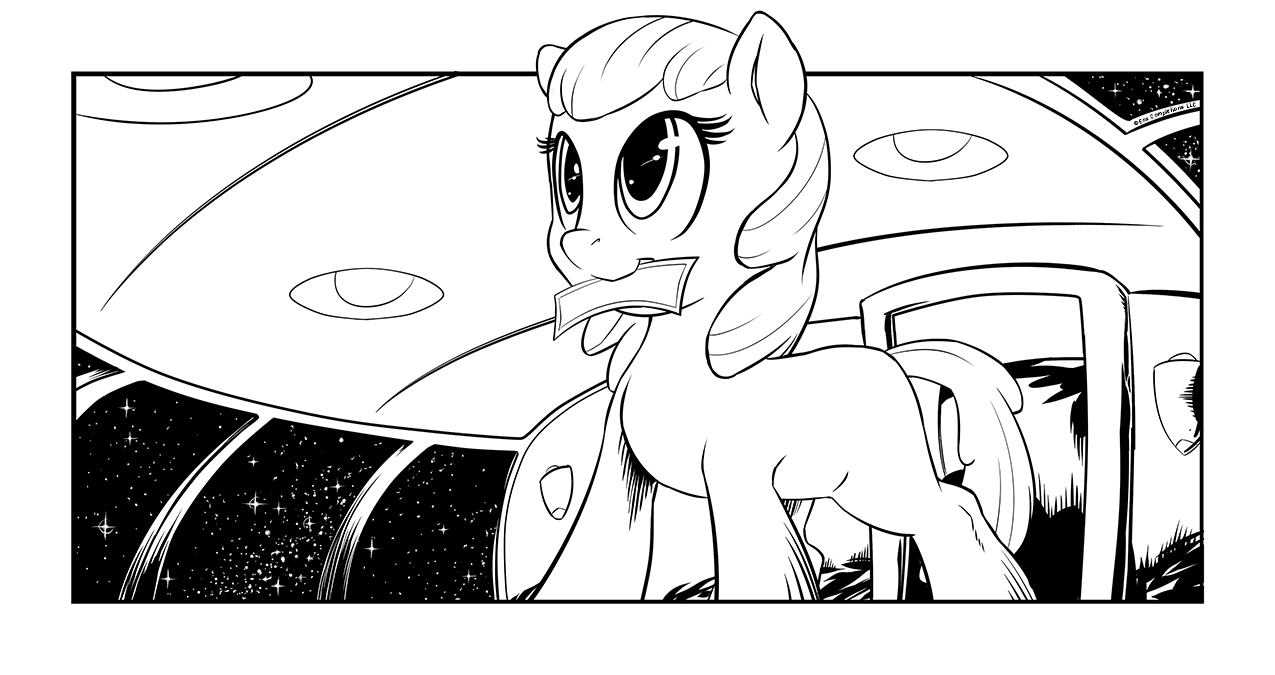
\includegraphics[width=0.9\linewidth]{image21.png}

\begin{intro}
    在那遥远的彼端,我们将再一次团聚。
\end{intro}

{\rt

「 拜托!别这样……滋滋……给我工作啊!」咣!咣!咣!「喂,喂,喂……测试测试……一二三……

「……

「好了,看起来没问题了,很好,我们开始吧,首先,我的名字叫守望者,我给自己的任务是守护整个废土,寻找那些在冒险中迷失的小马,希望能够找到那些带着谐律之源美德的小马。不过现在不一样了,我有很多朋友帮我的忙,我再也不孤单了,所以我终于有时间做我之前早应该做的事情。

「这就是我录这个磁带的原因,不过这一次,我希望你们叫我『提问者』。这个故事看起来不是那么重要,甚至有些傻里傻气,不过这个故事是关于梦与回忆的故事,是一个关于一双天真无邪的大眼睛的故事,那是一双即使看到现实的残酷,也坚信在这这片废墟之上,在那些奴隶营之中,甚至那些强盗的营地里面,每一个小马都还是漂漂马的大眼睛。

「而在她旅途的终点,当道路终于将她带到海边,迷失的小幽灵终于找到了安息之地。虽然她安息得稍微有那么一点迟,不过大家都说,她最终接受自己的命运的时候,是含笑离去的。

「这个小雌驹就像是来自战前的旧海报一样,她给52号国道上遇到的每一位小马带去了明媚的阳光,改变了他们如何看自己的方式,让他们看到一条更美好的道路,让他们更加期待明天。她并没有想要改变这个世界,或者拯救生命,但是她却引起了很多小马的关注。她自己并没有想当一个布道者,因为她显然不属于任何宗教或者派系也没有什么奇怪想法。她只是一个孩子,一个有着一对大大的粉色双眸的小孩子,她坚信着,众生天性本善。

「这些,这些就是帕比到达翡翠海岸之后又发生的故事。

「在野牛帮被击退之后,翡翠海岸的居民回到了他们的城镇。当他们从NCA过来的时候,他们发现那海岸边山丘上的新墓碑,还有倒塌的摩天轮。那景象确实让他们大吃一惊,在那之后不知道谁改了那个小镇的名字,现在那里叫做梦魇陨落。

「在新邻居的帮助下,铁砧镇的幸存者开始重建小镇,既然这里缺乏成年马,所以铁骑卫决定在这里定居下来,把这里当做他们的新总部。虽然不是所有小马都满意,不过铁骑卫用行动证明了自己对小镇的价值,之后就算最保守的小马也接受了他们。

「象牙塔和铁砧镇被摧毁之后,花椰菜那里迎接了无数流离失所的难民,那里的田地被扩大了好几倍,而且那里的农夫也提高了他们种田的技术。为了孩子们的快乐,他们现在不只种花椰菜,还种起了卷心菜。

「象牙塔现在的深坑已经被雨季的雨水填满,形成一个小湖,很多在花椰菜和铁锈庄园之间来去的行商在这里建立了一个临时落脚点,这里扩张得很快速,虽然到现在都没有一个名字,不过已经有一些行商叫这里『弹坑镇』。

「铁锈庄园在之后的英克雷入侵中饱受摧残,那里的机场控制塔都被炸毁了,很多小马都在战斗中牺牲。但是幸存者已经开始重建他们的家园,虽然那并不轻松,但是在废土之上没有什么事情是轻松的。

「太阳城现在还是个战区,因为聘蹄在英克雷入侵中离开了太阳城并且再也没回来,所以现在清砂帮和很多小帮派在都争夺这个沙漠明珠的控制权,这里还是个危险的地方,很多商队都绕道而行。不过对于那些敢于冒险的小马,城里随处可见的战前科技会让他们一夜暴富。

「隧道镇两边的城镇都扩张了好几倍,现在是52号国道第三大城市。隧道镇的隧道通行费现在变得很便宜,而且城市的卫兵开始在沿途进行巡逻,赶走了领土上所有的强盗和奴隶贩子。

「盐块城依然是52号国道最大的城市,而在那些尸鬼离开圆顶之后,城市更加发展壮大了。聘蹄的名声甚至远扬52国道之外,而且开始接受其它城市的任务了,虽然鹰爪并不太喜欢他们的新政策,不过两个佣兵势力之间的紧张关系正在慢慢升温。

「赤兔是改变最少的,他们依然保持着部族的传统,依然在他们的领土上游牧,不过幸运的时候,他们的孩子们可以自由地玩耍了。另外虽然不是什么大改变,部族现在也开始和其它城市合作了,并且在道路沿途设立定居点,让道路现在变得更安全。

「至于野牛帮,他们似乎在重创之后消声觅迹了,不过大家都知道他们总有一天还会卷土重来。但即使他们下一次再袭击52号国道,也不会有机器大军的帮助了,所以很长一段时间之内,小马们晚上都可以安心入睡。

「那些帮助铁砧镇重建的阿杰铁骑卫把他们的新基地建立在了铁砧镇的避难厩里面。在守护巢穴的战斗中,四位幸存的帕拉丁都来帮我守护这里,我有幸见到了冷浴和诘责,很可惜冷浴在那场恶战之中壮烈牺牲,她现在和她的朋友高斯一起长眠在翡翠海岸。诘责在失去她之后更加孤僻了,好像老书记官认为自己才是给朋友带来厄运的小马……我深深地理解他……

「乐乐和老枪结婚了,而且听说她怀孕了,这是最近才听到的消息,不过他们似乎并不想这么快就大张旗鼓地庆祝,不过我问起他们打算给小孩起什么名字的时候,乐乐看起来还没拿定主意,不过肯定不会是快乐帕比。

「融金在梦魇一战之后并没有停下他的传奇旅程,那尸鬼在康复之后就马上登上一艘航向南方的船,和一群冒险家一起探索新的大陆,不过在那之后我就没听说过他的传闻了。

「旭日系统和萍琪七号最后真的变成朋友了。我在第一次英克雷进攻之后联系到了P7,她很好奇这个帕比经常提到的『提问者』,所以我们聊了很久,虽然我还是不太信任她或者旭日OS,但是我觉得他们至少一段时间内不会给我们带来麻烦。不过她最后跟我说的一件事把我吓坏了,她似乎打算和旭日OS共同编写一个新的自律智能,并且起名为欢乐帕比\footnote{欢乐帕比:Puppy.~SML}……我希望这最好是个玩笑。

「孤狼在伤好之后继续经营他的52电台,继续用他的声音和音乐鼓舞着52号国道上的每一位居民,DJ好货也和他一同工作,不过我问他们打算什么时候结婚的时候,他们都在嘲笑我。在英克雷袭击中,52电台也一直持续工作,这个电台帮助52号国道组织起一次又一次反攻,并且极大地鼓舞了小马们的斗志,虽然并不是很大的帮助,但是足够让整个52号国道的居民打败了入侵者。

「白先生回到了盐块城之后,灌木的去世似乎让他受伤很深,即使她的妹妹并没有责怪他,但是他却不停地自责。之后他放弃了他的领导位置,变成一个旅行商,他现在依然在52号国道大路上来回行商贩卖着各种货物。不过有个传闻,据说他的秘书是一个有着白塔可爱标记的独角兽雌驹。或许他觉得雇佣一个有胆量打梦魇之月屁股的雌驹是一件很拉风的事,或许他只是想给一个强盗第二次机会……对吧?

「在长耳去世之后,她们部落又有一个新雌驹得到了先知的可爱标记。我不知道她们那神秘魔法是怎么弄的,不过用六种强力毒品混合出的迷幻药绝对会很快摧毁一个雌驹的身体,所以每次都需要有一个小马为部族而献身。

「赫瑞塔依然在四处躲藏着鹰爪的追杀,看起来他们和火红家族之的裂隙暂时无法弥补。那只年轻的狮鹫继续着家族的传统,我和高纳德聊过,看看能不能商讨出一个停战协议,毕竟她是帕比最好的朋友,如果看到她什么大事都没有做成就死于鹰爪的追杀,那实在太可惜了。

「幽灵羊群似乎已经完全消失了,在小跟班死后,每一个可怜的小灵魂似乎都终于安息了,小马国也可以愈合那场战争造成的众多伤痕之一,希望那些小家伙在来世之中找到他们的归宿。

「不过还有一个小马我从来没有见过,而且我甚至开始怀疑他是否存在,帕比跟我说他可是……她所见过的最坏坏蛋,马尾伯爵,我问了很多旅者和车队卫兵,不过看起来没有谁对这个残酷的贵族小马有什么印象……我觉得或许将是个永远无法解开的谜团。

「好了,这就是帕比故事的结局了,她真的在旅途之中改变了什么吗?她这场长长的冒险真的有意义吗?抱歉,我也不知道,不过我想我会怀念她的,在她看来,一切都如此简单。随着她的去世,另一片来自战前小马国的碎片也永远随风而逝。不过我希望今后有一天能够再次见到和她一样天真无邪的孩子,希望这一次不是来自过去的幽灵,而是某对真实夫妻的女儿。

「说到幽灵,52号国道的幽灵传说依然在继续,而且现在听起来更像是梦魇夜的鬼故事。据说在太阳落山,月亮升起来之后,一个无声的幽灵会随风在大路上游荡,它会夺走那些坏孩子的灵魂。那些奴隶贩子,那些强盗,甚至那些心怀恶意的家伙,他们身上没有一点伤口,武器依然上膛,但是他们却都已经死了,完全不知道被什么东西袭击,一点线索都没有。所以,我只想问你一件事。

「你相信幽灵么?」

}

\horizonline

\daytimeplace{4}{7:30 PM}{闹市区,盐块城}{Downtown, Salt Cube City}

沙盒用力按着船舵,让飞空艇迎风飞行,不过看起来完全不可能。友谊一号正在慢慢地失去他们起飞的速度,两个引擎已经熄火了,尸鬼用蹄子猛砸内部通话系统的开关,然后喊道:「软气,我们需要更多动力!我们正在被夜风吹回去!我不知道怎么做,不过再快几节行不行!」

话筒里传来带着静电沙沙声的回答,听起来似乎是气球正在漏气还有引擎起火啥的。

沙盒咒骂着,然后再一次怒吼起来。

「好了,别担心,我还有另外一个计划,我们让这个空艇就在这里坠毁,这样夜风就不会把我们吹回盐块城了!」

不过那一边的回答沙盒并没有听到,因为这个时候整个世界都被一道亮光洗白了。

无穷无尽的炫目光明掩盖了一切,没有痛苦,没有恐惧,只有光明。

\horizonline

\unknowndaytimeplace

当沙盒再一次睁开眼睛的时候,他微妙地感觉到有什么不对劲——应该说没有任何『不对劲』。他环视着舰桥,想搞明白到底出了什么事。船舵还在那里,外面的天空繁星闪闪,指令舱一切正常,灯泡也全亮……{}

「等等……灯泡怎么全好了?外面的星星是怎么回事?到底是……」

没错,飞艇运行得非常良好,比那整个拱顶塌下来,它飞出空港的时候都要好!地板闪闪发光,指令台擦得锃亮,甚至舵上还打了蜡!还有窗户,都擦得如此洁净,甚至可以看得见自己的……{}

然后沙盒看到了自己那吃惊到发傻的表情,他慢慢的伸出蹄子碰了碰自己,那是……他自己的脸,真正的脸,在他变成尸鬼之前的脸!他又是小马了!他……{}

死了。

他死了,这是一切唯一合理的解释。但如果他死了,为什么还在这艘船上?难道是某种死后世界的惩罚,他必须永远开着这艘飞艇,就像是加勒比海马一样?其他小马也和他一样永远困在这艘船上了么?为什么?他才不要永远飞这东西!他要见阿加莎!她……她肯定某处等待着他……他不能就这样……就这样开着一艘破船到处漂流!

一声明亮的口哨打断了沙盒的鬼船猜想,把他的视线拉回了舰桥入口,一只雌驹推开舱门大喊,她的嗓门又尖又高,刺得沙盒鬃毛都竖了起来。

「船长驾临舰桥\footnote{船长驾临舰桥(CAPTAIN ON THE BRIDGE):星际迷航名句}!」

有双蓝色大眼睛和粉色卷毛的粉色雌驹蹦跶到了前尸鬼面前,她穿着一身海军军官制服,脸上还带着沙盒从来没见过的大大笑容。

「萍……额……派部长?」

萍琪并拢双蹄行了一个军礼,「喏,叫人家萍琪船长就是,才不喜欢那些政治杂务……一点都不有趣!」年轻的雌驹在舰桥上蹦来蹦去,疯疯癫癫地咯咯笑着打滚,「耶!我就知道这孩子迟早能飞上天!哦哦哦哦!你看这个,所有的仪表盘都是粉色,和我要的一样!简直太妙了!」

首席技师满脸莫名其妙地看着那神经兮兮的雌驹用他眼睛都跟不上的速度在船上碰这碰那。

「呃……有什么我可以效劳的么?」

还没把话说完,沙盒就发现萍琪已经跳到了他面前,自己正在和萍琪那对蓝蓝的眼睛小眼瞪大眼。

「当然有!他们早就在沙龙等亲了!快去下面参加派对吧!等我在这儿玩够了就下去!」

那公马点点头,一边慢慢后退到门口,一边紧紧盯着萍琪。感觉她稍微有点可怕,特别是在一个刚刚死了没有十分钟的小马眼里。等蹄子踩上楼梯的时候,他急忙调转尾巴飞快地离开舰桥。

下面的沙龙虽然不是挤得满满当当,但是依然算是热闹非凡。沙盒明明记得友谊一号起飞的时候只载了四个乘客,但是现在他却看到八个宾客。

他很容易就认出了穿着飞行员制服的软气,桃花的那个绽放桃花可爱标记也很好认,在他们俩身边的那个中年雌驹应该就是好好医生,不得不说,她的皮肉都在身上的时候真的很有风韵。而另外一边的那个狮鹫和另外四只小马,沙盒就不认识了。

狮鹫正坐在沙发里面看着报纸喝茶,他穿着一件防弹衣,上面挂着好几把武器。另外两只小马——一公一母马,都穿着动力装甲下面的战术衬垫服,正在肩并肩站在桌子旁边吃着点心。他们其实并不太关心桌子上的东西,而是时不时地互相磨蹭着对方,看起来相当恩爱。

第三只小马则坐在窗边,忧心忡忡地看着窗外,一个劲儿地叹气。他的眼神中有太多的后悔和留念,看起来他对世界还有太多眷恋,并不想走。而第四只小马是穿着长披风的独角兽雌驹,她带着清砂帮的珠宝饰物,或许她是个先知什么的?那个雌驹看起来和其他小马完全不同,似乎只是个影子而不是真实的存在。不过她看到沙盒走进屋子里面就立刻站起来迎接他。

「您好,看起来萍琪最后还是把你叫下来了,看起来我们已经可以继续了……我想她很快就会来这里了,除非她又迷路了。」

沙盒皱起了眉头,「继续什么?她是谁,你又是谁?我说,我不是来找麻烦的,但是……」他的话被一阵小小的蹄声打断,一只有着大大粉色双眼,金色鬃毛的粉色小雌驹跑进屋子里面。

帕比在嘴里紧紧衔着她的那张银色机票,她不太清楚自己怎么来到这个地方的,不过没关系,这里有游戏,有吃的,看起来绝对是个超级华丽的派对!这是她一直梦想的一切,而且这里面都是小马,还有个小鸡!

沙盒觉得自己的心开始往下沉,在死后想见到的所有小马里面,他最不想见到的就是快乐帕比。「哦,小家伙……我……我……很抱歉……」为什么这孩子现在还能露出这样灿烂的微笑?「发生什么了?是谁……你怎么到这里的?」

帕比微微歪着头,似乎没有认出来面前的是谁,不过他看起来很友好所以没关系。

「嗨!漂漂马先生!我叫快乐帕比!我马上要见到妈妈了!一个超级好的骷髅马给了我这张超级厉害的机票然后把我送过来了!而且他说我马上就可以看到妈妈,就在降落之后!」小雌驹顿了顿,看了看窗外。「我们还没到么?」

沙盒眨了眨眼睛,想明白那孩子到底在说什么,不过长耳走过来和他咬耳朵,「她的妈妈已经死了……」但是这只是让沙盒更混乱了。

「你……你死了很高兴?」

帕比咯咯笑着,「那个骷髅马也这么问我,不过我现在觉得很开心因为我马上就能见到妈妈了,这就像是……像是……最好最好的事情!」

「但……但是……」她是那么快乐,即使是她已经知道将要发生什么,不过,有什么好不开心的么?沙盒想到这里微笑地掉了点头。

「对,没错,降落之前你想和我们玩游戏吗?」

在他们聊天的时候,房间里面的小马已经慢慢聚集到了帕比身边,他们看着那小雌驹,视线里都带着一丝歉意和一丝悔意。冷浴和高斯走到小雌驹身边,那母马先开口了。「很抱歉我们必须和你一战……我真希望我们有更好的办法……」高斯也点了点头,深深叹了口气。

「哎?为啥大家都那么伤心?为什么不玩游戏?我要玩捉迷藏!或者钉马尾!或者大家一起来跳舞也可以!哦哦哦……钉马尾的马尾要粉色的!因为粉色是我最喜欢的颜色!我可是最厉害的钉马尾大师!」看到这么多小马围过来,帕比乐得一蹦三尺高。

不知什么时候换上了一件空姐制服的萍琪从帕比进来的那个门走了过来,拍了拍小雌驹的头,「很抱歉帕比,没时间做游戏啦!因为我们已经到达了星之海的彼岸!现在我们已经降落啦!旅途到此结束,女士们,先生们!感谢你们选择天堂航班!祝你们旅途愉快!」粉色雌驹飞快地跑到门口打开舱门,而舱门外是一片绿茵盎然的境外桃源美景。

一群群小马在草地上悠闲的散步,天马坐在蔚蓝天空中的朵朵白云上。飞船的旅客登机梯伸展下去,落在了这片美丽的大地上。这里看起来就像是美梦成真一样,远处还能看到一片片美丽的果园和一幢幢平整的房屋。

即使是帕比也被面前的美景惊得说不出话来,那些树木,那些草地,还有那么多漂漂小马和美丽的蔚蓝天空……这比……这比小马镇都要棒!这里如此美妙,唯一缺的就是……

帕比愣了一下,她望着那一小群朝飞空艇走来的小马,脸上的微笑越来越灿烂。她跳下飞船飞奔在草地上。迎面飞奔而来迎接她的,是一只同样喜极而泣的雌驹。帕比开心得什么都说不出来,唯一能大声喊出来的,就是——

「妈咪!」



